
\documentclass[12pt]{report}

\usepackage{fullpage}
\usepackage{graphicx}
\usepackage{listings}
\usepackage{verbatim}
\usepackage{amsmath}
\usepackage{color}
\usepackage{hyperref}
 
\definecolor{codegreen}{rgb}{0,0.6,0}
\definecolor{codegray}{rgb}{0.5,0.5,0.5}
\definecolor{codepurple}{rgb}{0.58,0,0.82}
\definecolor{backcolour}{rgb}{0.95,0.95,0.92}
 
\lstdefinestyle{mystyle}{
    backgroundcolor=\color{backcolour},   
    commentstyle=\color{codegreen},
    keywordstyle=\color{magenta},
    numberstyle=\tiny\color{codegray},
    stringstyle=\color{codepurple},
    basicstyle=\footnotesize,
    breakatwhitespace=false,         
    breaklines=true,                 
    captionpos=b,                    
    keepspaces=true,                 
    numbers=left,                    
    numbersep=5pt,                  
    showspaces=false,                
    showstringspaces=false,
    showtabs=false,                  
    tabsize=2
}

\lstdefinestyle{DOS}
{
    backgroundcolor=\color{black},
    basicstyle=\scriptsize\color{white}\ttfamily
}
 
\lstset{style=mystyle}
\renewcommand{\baselinestretch}{2}
\author{Mohammed Nauman Siddique}
\title{Assignment 5 \\Information Retrieval \\ CS 834 \\ Fall 2017 }

\begin{document}
\maketitle
\tableofcontents
\chapter{Problem 10.3}
\section{Problem Statement}
Compute five iterations of HITS (see Algorithm 3) and PageRank (see Figure 4.11) on the graph in Figure 10.3. Discuss how the PageRank scores compare to the hub and authority scores produced by HITS.
\section{Solution}
The page ranks and authority, hub values for hits algorithm are based on the below directed graph. 
\begin{figure}[ht]
  \centering
  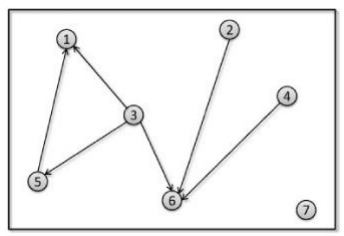
\includegraphics[width=1\textwidth]{Problem10_3/Graph.png}
  \caption{Directed graph for PageRank and HITS algorithm}
  \label{fig:1}
\end{figure} 
\subsection{PageRank}
PageRank for the graph has been calculated by assuming the initial pageranks for all the pages to be equal to reciprocal of the number of nodes. The detailed description of the pageranks per iteration is available in the tables below.
\subsection{HITS Algorithm}
The initial values for hub and authority for all the pages was initialized to 1. The authority and hub values per iteration is in the tables below.

\begin{table}[]
\centering
\caption{PageRank, Hub and Authority Values after Iteration 1}
\label{my-label}
\begin{tabular}{llll}
Node & PageRank            & Hub                 & Authority           \\
1    & 0.18333333333333332 & 0.0                 & 0.3333333333333333  \\
2    & 0.14285714285714285 & 0.16666666666666666 & 0.0                 \\
3    & 0.14285714285714285 & 0.5                 & 0.0                 \\
4    & 0.14285714285714285 & 0.16666666666666666 & 0.0                 \\
5    & 0.06190476190476191 & 0.16666666666666666 & 0.16666666666666666 \\
6    & 0.30476190476190473 & 0.0                 & 0.5                 \\
7    & 0.14285714285714285 & 0.0                 & 0.0                
\end{tabular}
\end{table}   

\begin{table}[]
\centering
\caption{PageRank, Hub and Authority Values after Iteration 2}
\label{my-label}
\begin{tabular}{llll}
Node & PageRank            & Hub                 & Authority           \\
1    & 0.11452380952380953 & 0.0                 & 0.33333333333333337 \\
2    & 0.14285714285714285 & 0.21428571428571427 & 0.0                 \\
3    & 0.14285714285714285 & 0.42857142857142855 & 0.0                 \\
4    & 0.14285714285714285 & 0.21428571428571427 & 0.0                 \\
5    & 0.06190476190476191 & 0.14285714285714285 & 0.25000000000000006 \\
6    & 0.30476190476190473 & 0.0                 & 0.4166666666666667  \\
7    & 0.14285714285714285 & 0.0                 & 0.0                
\end{tabular}
\end{table}

\begin{table}[]
\centering
\caption{PageRank, Hub and Authority Values after Iteration 3}
\label{my-label}
\begin{tabular}{llll}
Node & PageRank            & Hub                 & Authority           \\
1    & 0.11452380952380953 & 0.0                 & 0.30769230769230765 \\
2    & 0.14285714285714285 & 0.1923076923076923  & 0.0                 \\
3    & 0.14285714285714285 & 0.46153846153846156 & 0.0                 \\
4    & 0.14285714285714285 & 0.1923076923076923  & 0.0                 \\
5    & 0.06190476190476191 & 0.15384615384615385 & 0.23076923076923075 \\
6    & 0.30476190476190473 & 0.0                 & 0.4615384615384615  \\
7    & 0.14285714285714285 & 0.0                 & 0.0                
\end{tabular}
\end{table}

\begin{table}[]
\centering
\caption{PageRank, Hub and Authority Values after Iteration 4}
\label{my-label}
\begin{tabular}{llll}
Node & PageRank            & Hub                 & Authority           \\
1    & 0.11452380952380953 & 0.0                 & 0.31999999999999995 \\
2    & 0.14285714285714285 & 0.20689655172413796 & 0.0                 \\
3    & 0.14285714285714285 & 0.4482758620689656  & 0.0                 \\
4    & 0.14285714285714285 & 0.20689655172413796 & 0.0                 \\
5    & 0.06190476190476191 & 0.13793103448275862 & 0.24                \\
6    & 0.30476190476190473 & 0.0                 & 0.43999999999999995 \\
7    & 0.14285714285714285 & 0.0                 & 0.0                
\end{tabular}
\end{table}

\begin{table}[]
\centering
\caption{PageRank, Hub and Authority Values after Iteration 5}
\label{my-label}
\begin{tabular}{llll}
Node & PageRank            & Hub                 & Authority           \\
1    & 0.11452380952380953 & 0.0                 & 0.3090909090909091  \\
2    & 0.14285714285714285 & 0.2                 & 0.0                 \\
3    & 0.14285714285714285 & 0.45454545454545453 & 0.0                 \\
4    & 0.14285714285714285 & 0.2                 & 0.0                 \\
5    & 0.06190476190476191 & 0.14545454545454545 & 0.23636363636363636 \\
6    & 0.30476190476190473 & 0.0                 & 0.4545454545454546  \\
7    & 0.14285714285714285 & 0.0                 & 0.0                
\end{tabular}
\end{table}

\section{Discussion}
A node with higher pagerank  is considered as a better result. A page with high hub value tells that it points good authorities. A page with high authority values tells that it is pointed by good hubs. Based on this idea, the results on the graph suggests that node 6 has the best page rank and best authority value. Both the techniques PageRank and HITS algorithm suggest node 6 to be most relevant to the query. Node 3 has highest value of hub suggesting it points to the best authorities. The node 7 which has no inlinks and outlinks has low pagerank, hub and authority value. The pages without any inlinks and outlinks have a hub and authority value of 0 but the page rank value is equal to the reciprocal of the number of nodes. 

\chapter{Problem 10.5}
\section{Problem Statement}
Find a community-based question answering site on the Web and ask two questions, one that is low-quality and one that is high- quality. Describe the answer quality of each question.
\section{Solution}
One obvious example of community-based question answering site is Stack Overflow. I have framed my understanding of low-quality and high-quality questions with the partial information provided in the book. Low-quality question refers to questions which are generic, grammatically incorrect or vague in their idea while the high-quality question refers to questions which are specific and well-structured. For this question, I have reused the questions I asked previously from my profile at Stack Overflow.
\subsection{Low-Quality Question}
I judged my question to be low-quality on the parameter of ill-structured formation of the question. The question had 466 views on Stack Overflow but no one answered to my query not because of the difficulty of the problem but due to the poor formation of question and vagueness in the idea of the question. I judged it later in time when I was able to fix the problem which I had asked on Stack Overflow by altering the question. When I went back and looked at my question I realized I had put forward a question without any context of the problem I was talking about. Although I never received a formal answer to my problem, but a lot of people did suggest me edits to my question to frame a high-quality question. 

\begin{figure}[ht]
  \centering
  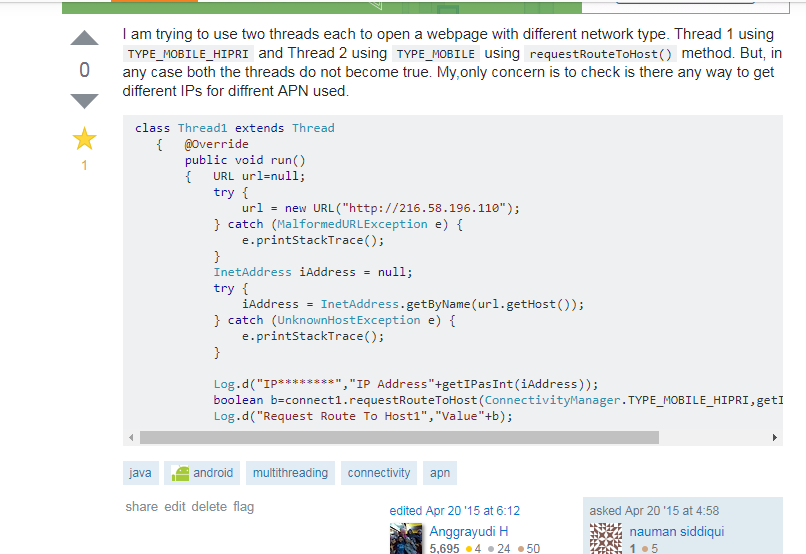
\includegraphics[width=1\textwidth]{Problem10_5/LowQuality.png}
  \caption{Screenshot of low-quality question}
  \label{fig:1}
\end{figure} 

\subsection{High-Quality Question}
I judged this problem to be high-quality on the parameters that it was a very specific question with a clear idea about the problem. I received an answer to my question asking me to debug the code with return status codes and a link to the linux man page of the function which helped me figure out for the odd behavior in my code. The answer quality for this question was very precise and helpful.   
\begin{figure}[ht]
  \centering
  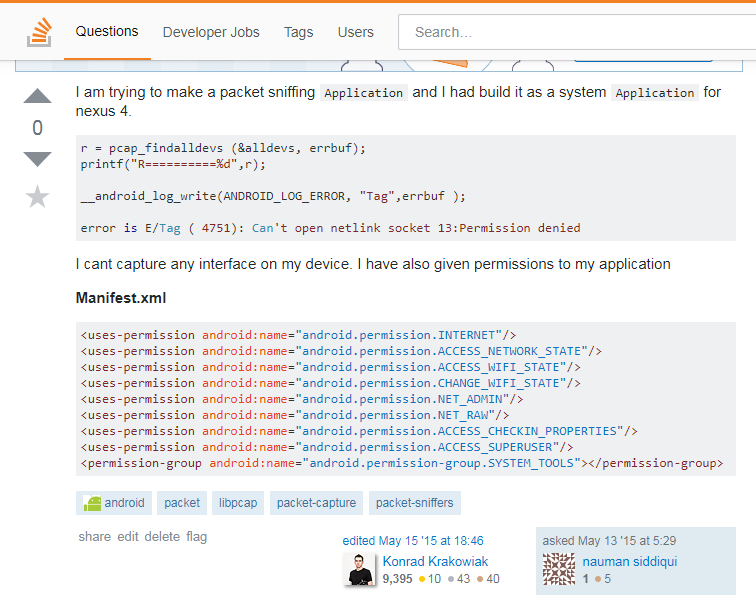
\includegraphics[width=1\textwidth]{Problem10_5/HighQuality.png}
  \caption{Screenshot of high-quality question}
  \label{fig:1}
\end{figure} 

\subsection{Summary}
A high-quality question shows the effort of the user who asks the question and clarifies his information needs making the community enthusiastic to help him solve the problem whereas, a low-quality question discourages the community in replying answers to the question which hurt the reputation of the user who asks the question and leading to lower probability of his questions getting answered. 

\chapter{Problem 10.6}
\section{Problem Statement}
Find two examples of document filtering systems on the Web. How do they build a profile for your information need? Is the system static or adaptive?
\section{Solution}
Document filtering systems provide a way for personalized search result for users on the basis of their information needs. Multiple services on the web serve the purpose of document filtering in present time.
\subsection{Stack Overflow}
Although it is a community-based question answering forum, it also serves as a good example for document filtering technique. It allows users to build subscriptions to information based on their preferences. It asks users to set their preferences by specifying the websites which are part of Stack Overflow community and further ask the users to specify the tags in which they are interested. On the basis of the information requirement provided to the service it alerts the users with email on the basis of the frequency set for receiving the email. It helps the user share their knowledge relevant to their area of interest and also with keeping up with the latest issues faced by other user's relevant to their area of interest.This is an adaptive system allowing using to change the filter parameters overtime to meet their requirements. Stack Overflow allows multiple filters to be created  by the same user to keep up with their varied variety of interest.  

\begin{figure}[ht]
  \centering
  \includegraphics[width=1\textwidth]{Problem10_6/Stackoverflow.png}
  \caption{Screenshot of Stack Overflow alerts builder}
  \label{fig:1}
\end{figure} 

\subsection{Google Alerts}
 It is a document filtering system because it allows its users to monitor their interests by creating alerts. It allows users to build alerts on the basis of their over all interest unlike Stack Overflow which is responsible for only technical interests. It has a page which suggests topics to the users and a search bar where the user can type in their interests. On the basis of the tags set for alert the Google alerts service provides alerts to the users via email each time a new news comes with the interest tag of the user in the headline. The service also shows the preview of the news articles relevant to the tags entered by them. It builds the users profile for information needs by asking multiple questions from the users like how often they want the news, the source of news, language of news. region specific, frequency of email to be sent. It is also an adaptive system allowing users to update their information needs over time. The users can update the detailed information about the topic but to change the topic of interest it needs to be deleted and a new filter needs to be created with updated topic of interest.

\begin{figure}[ht]
  \centering
  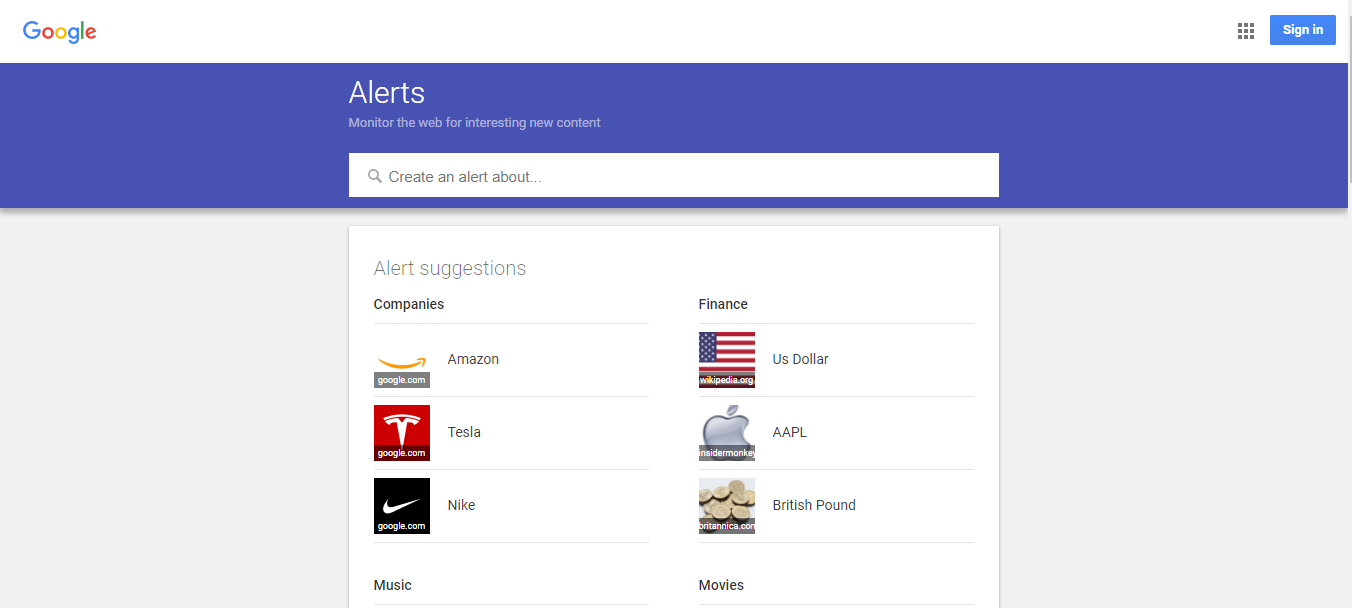
\includegraphics[width=1\textwidth]{Problem10_6/GoogleAlerts.png}
  \caption{Screenshot of Google Alerts}
  \label{fig:1}
\end{figure}  

\subsection{Summary}
The web has multiple document filtering system which can be static or adaptive. Most of the job search websites, news websites etc. support this feature allowing users to receive information about their topics of interest. In my evaluation I used both the services which build adaptive profiles allowing users to update their information needs.

\chapter{Problem 11.9}
\section{Problem Statement}
Find a demonstration of a question answering system running on the Web. Using a test set of questions, identify which types of questions work and which don’t on this system. Report effectiveness using MRR or another measure.
\section{Solution}
The easiest way to find answers to questions is Google but it presents us with ranked list of documents and not an answer as a human replies to questions. Although there are many question-answering services online but they are focused on a particular topic. So, I chose START, a Natural Language Question Answering System built by MIT. It returns answers to questions that are very similar to humans. The system returns answer to the question in case of a hit and returns no answer in case of a miss. While in case of Google, either in case of a miss or hit it mostly presents us with a list of relevant documents  which match our query and finding the answer is the user's responsibility. 
\subsection{Analysis of START}
The sample queries used to test the system were mostly reused from the TREC sample questions provided in the book in Table 11.2. For analysis I tested the system on games, geography, politics, chemistry and computer based  questions. The questions were mostly low-level questions because of their generic nature.
Few Sample Question:\\
1. What is the capital of India?\\
2. What is the difference between soccer and football?\\
3. Who is the governor of Virginia?\\
4. What is the latest version of python?\\

\begin{figure}[ht]
  \centering
  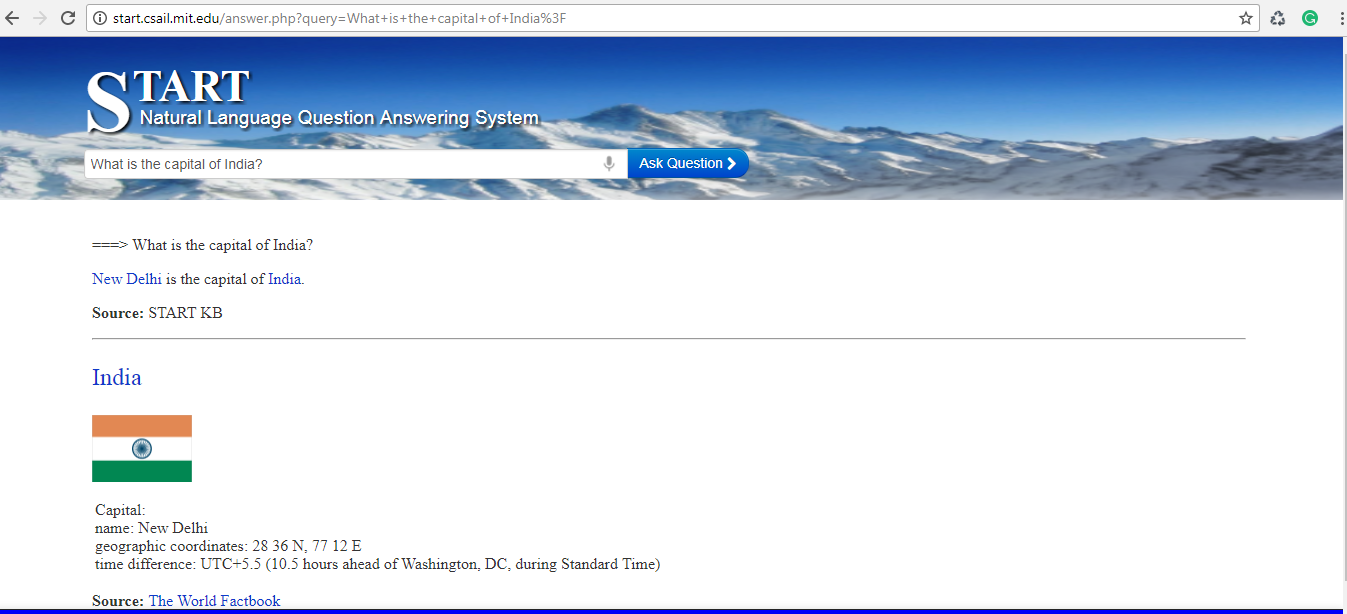
\includegraphics[width=1\textwidth]{Problem11_9/Delhi.png}
  \caption{Screenshot of Answers returned}
  \label{fig:1}
\end{figure} 
 
\begin{figure}[ht]
  \centering
  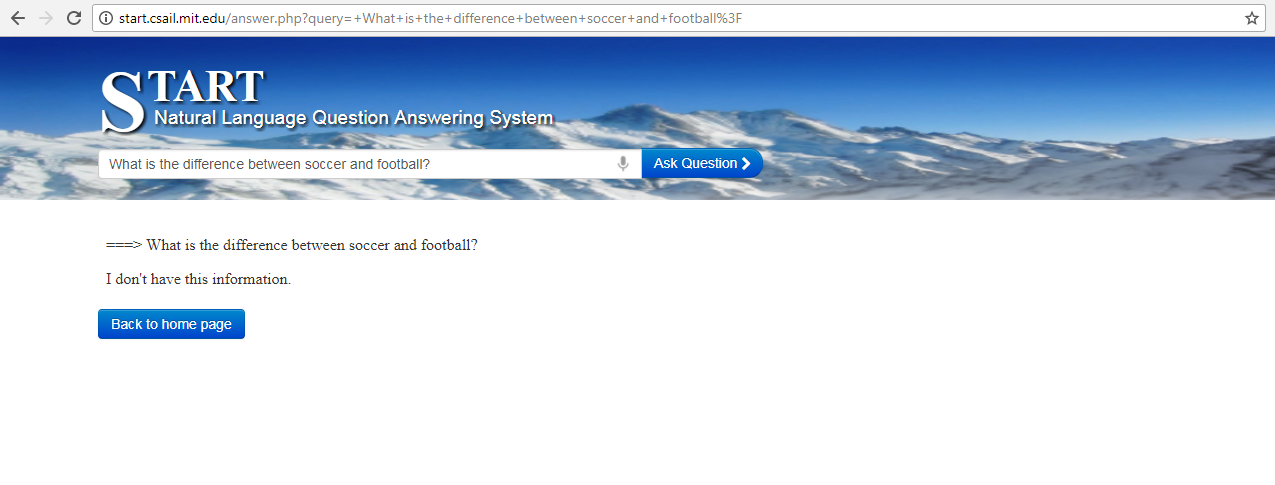
\includegraphics[width=1\textwidth]{Problem11_9/NoAnswer.png}
  \caption{Screenshot of Answers not returned}
  \label{fig:1}
\end{figure} 
The system returns answers or does not return if no answers are found. The effectiveness of the system can not be measured by MRR because the returned result is an answer rather than a list of documents with a ranking. The measure of precision and recall will be 1 in case of answer returned else it will be 0. So, to effectively measure the system we could use a modified version of recall which will be sum of all the recall values for queries divided by the number of queries.\\
$Recall = (\sum\limits_{i=1}^N Recall_i) /N$\\
where,\\
N is the total number of queries\\
$Recall_i is the recall value for query i$ \\
For my analysis I ran 20 queries with 4 questions from each category named earlier. The system returned answers to 11 questions out of 20 making the  average Recall for the system to be 0.55. The system answers questions which are fact based but a semantic-based question has no answer in the system. An example of semantic-based question is What is the difference between soccer and football which required the system to have a better understanding of its corpus rather than a tf.idf approach to answering the questions. 
\chapter{Problem 11.11}
\section{Problem Statement}
Look at a sample of images or videos that have been tagged by users and separate the tags into three groups: those you think could eventually be done automatically by image processing and object recognition, those you think would not be possible to derive by image processing, and spam. Also decide which of the tags should be most useful for queries related to those images. Summarize your findings.
\section{Solution}
I am using Flickr to find images which are human tagged and classify them as tags which can be generated by image processing, tags which can not be generated by image processing and spam.
\begin{figure}[ht]
  \centering
  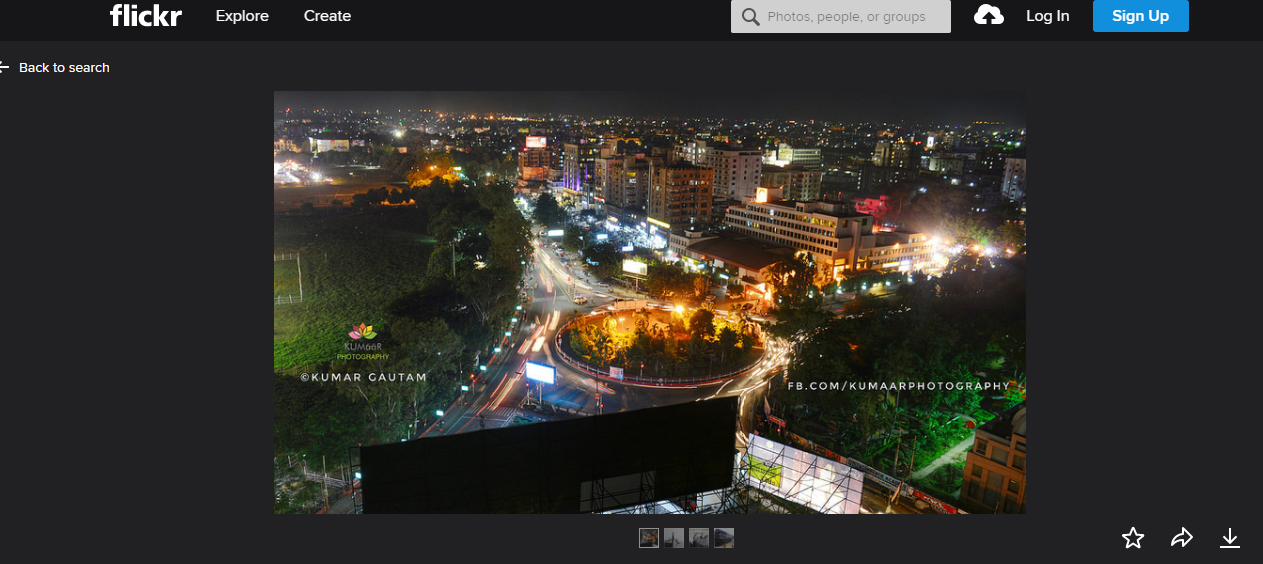
\includegraphics[width=1\textwidth]{Problem11_11/HumanTag.png}
  \caption{Screenshot which can have image processing generated tags (Tag for image: Light trails View of Patna(Bihar) /\#patna \#gandhimaidan \#lighttrails \#nightphotography)}
  \label{fig:1}
\end{figure}

\section{Determining nature of tags}
The tags have been classified as a human tag by analyzing the tags attached to the image.  The screenshot displaying human generated tag in Figure 5.1 is of my hometown Patna. The image tag can be generated by image processing and object identification technique because of the unique buildings in the image. The image processing systems in Google would have come across multiple images on the same place tagged with the relevant tags to make it easy for their system to identify this image is of Patna.The image can also be tagged automatically by learning from prior experience and not by simple object identification. The tag for the image has a number of tags relevant to the image but still a few more tags could be attched to the image regarding the remaining landmarks visible in the image and out night photos of Patna which would make the image very relevant for queries searching for this image.\\
\begin{figure}[ht]
  \centering
  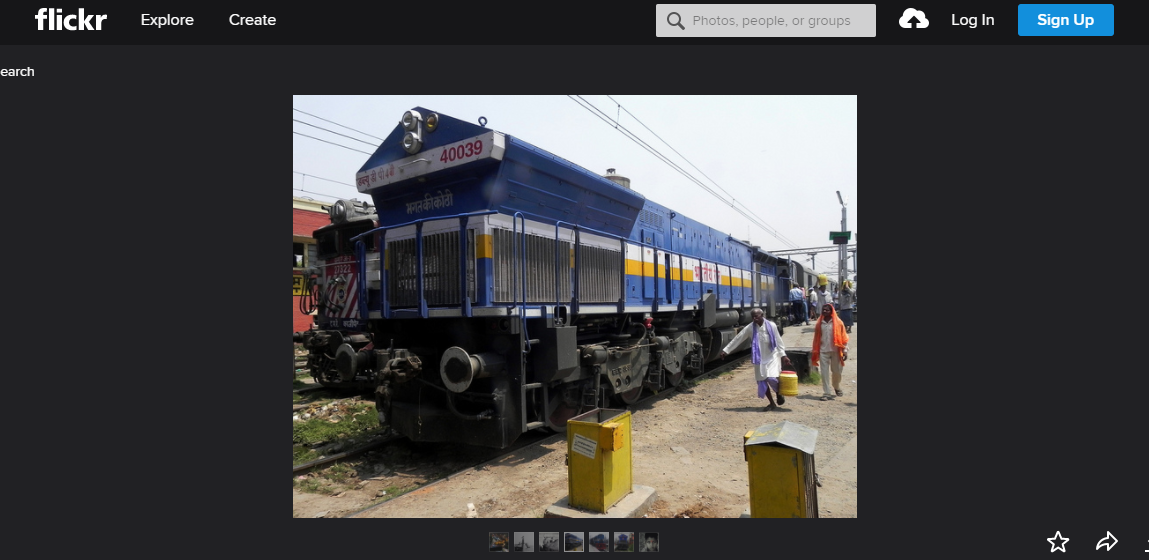
\includegraphics[width=1\textwidth]{Problem11_11/Spam.png}
  \caption{Screenshot of spam tag in images (Tag for Image: Sharanjeevi Express)}
  \label{fig:1}
\end{figure}
The image in figure 5.2 was judged as a spam because it is a very generic image of a locomotive engine and the tag of the image does not make any sense to the image. The tag for the image tells name of a particular train which it could be and not be, so the perfect tag for this image would be a locomotive engine, WDP4 locomotive or Indian Railways.\\
\begin{figure}[ht]
  \centering
  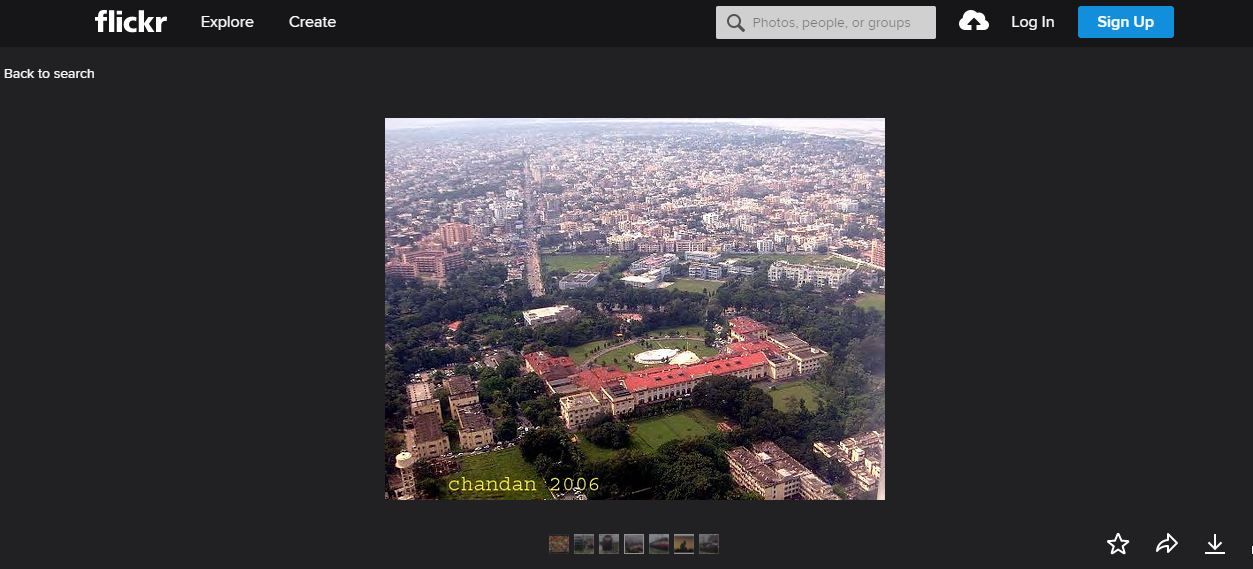
\includegraphics[width=1\textwidth]{Problem11_11/HumanTag1.png}
  \caption{Screenshot which cannot have image processing generated tags (Tag for image: Patna High Court))}
  \label{fig:1}
\end{figure}
The image in figure 5.3 was judged to category of images whose tags cannot be generated by image processing and object identification because of the aerial view of the image. The view of the image makes it very generic and redundant for systems to uniquely identify the landmark and can only be tagged by a human who knows the place by figuring out patterns in the image. The tags in the image could be added to indicate of aerial view of Patna city and the landmark tagged with it to make it more relevant for multiple versions of queries searching for Patna High Court or Patna city.\\
\begin{figure}[ht]
  \centering
  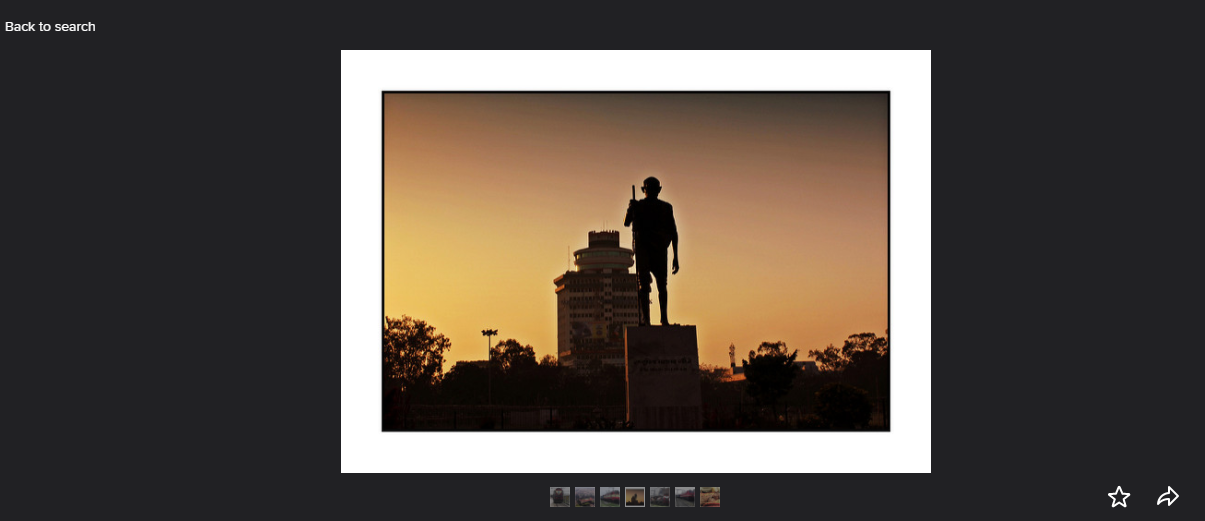
\includegraphics[width=1\textwidth]{Problem11_11/HumanTag2.png}
  \caption{Screenshot which cannot have image processing generated tags (Tag for image: Vande Mataram))}
  \label{fig:1}
\end{figure}
The image in figure 5.4  judged to category of images whose tags cannot be generated by image processing and object identification because of the vagueness of human generated tag with the image. An automatic image processing system would tag the image for the statue and the building visible in the image making it more relevant than the human tag. For the current human tag, it is a nationalism slogan which cannot be used in statue image of Mahatma Gandhi. The tags about the statue and building visible in the image and also predicting the city would make this image more worthwhile for query search.
\subsection{Analysis}
I analyzed most of the location based images which are easy for image processing systems to identify with the relevant human tags based on the features present in the image, but it is not possible in all the cases. A number of images which have a vague human generated tags make the image useless and can be made useful by the automatic tag generation of image processing techniques. Human generated tags also make a image spam which can be identified by a system because the image contains no relation with the human generated tag. Human generated tags are useful in identifying images but cannot be relied 100\% because of the casual nature of humans making images mean something else which they truly are not. \\
With most of the location images available on Google maps it has become very convenient for image processing systems to train on those images to predict the tags very accurately to an image unless the system is not trained with flawed human tagged images.

\chapter{Problem Extra Credit SVMLight}
\section{Problem Statement}      
Extra Credit: SVMlight, 10 points extra credit:
see: $http://www.cs.cornell.edu/People/tj/svm_light/$
* 1 point:
work through the "Inductive SVM" example, discuss in detail the steps and resulting output
* 9 points: 
- create your own example modeled after the "Inductive SVM" example
- pick a topic (e.g., "Australia") and provide 100 positive and 100 negative examples for training data:
  -- using the Reuters-21578 collection (linked from the SVMlight page)
  -- or, create your own collection with crawled web pages 
- pick 30 documents not in the training set for your test data
- stem the words in the collection, using TFIDF as the features (compute for the 230 documents)
- train, classify, and discuss the results
\section{Solution}
The SVMLight has two modules svm learn and svm classify. SVM learn is used to  train and classify the dataset and produce a model file which contains all the support vectors. SVM classify is used to apply to the model files to measure the accuracy the classification of  the training dataset on running against non-trained data. SVM learn reads all the examples and sets the value of  regularization parameter (C) to be 1. The value of regularization parameter decides how much of misclassification is acceptable for the training data. A large value of C does a better job at classifying data points while a small value will have a lesser accuracy in classifying points. It prints the value of misclassified points for the training data based on the default value of C equal to 1. it also mentions about the number of support vectors used for training the data.L1 loss function is basically minimizing the sum of the absolute differences (S) between the target value and the estimated values. It mentions the values for L1 loss function. It also generates estimated VCdim of the classifier. VCdim measures the capacity of a hypothesis space. Capacity is a measure of complexity and measures the expressive power, richness or flexibility of a set of functions by  assessing how wiggly its members can be.  It also generates values for computes XiAlpha-estimates of the error rate, the precision, and the recall. SVM classify reads all the classified support vectors of the training dataset to predict the accuracy of the untrained dataset provided to the SVM with the and the precision and recall values for the new dataset.

\begin{figure}[ht]
  \centering
  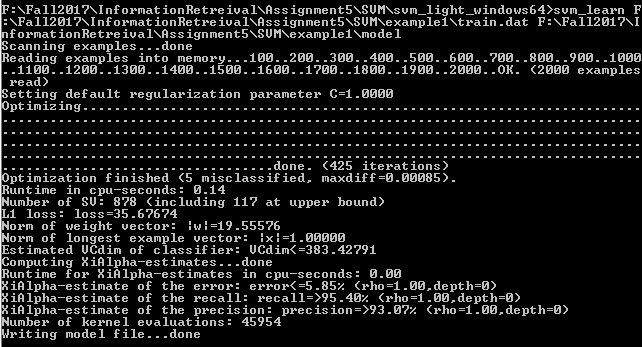
\includegraphics[width=1\textwidth]{SVM/svm_learn.png}
  \caption{Screenshot of svm\_learn command on the example dataset}
  \label{fig:1}
\end{figure}

\begin{figure}[ht]
  \centering
  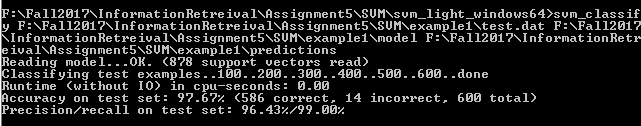
\includegraphics[width=1\textwidth]{SVM/svm_classify.png}
  \caption{Screenshot of svm\_classify command on the example dataset}
  \label{fig:1}
\end{figure}
\end{document}